\chapter{Design}

This chapter covers the architectural design of the proposed system for integrating Apache Ranger as an access control system for OpenMetadata. It lays out the high-level structural components, details the protocol these use to communicate and outlines the approaches used. Comprehensive details of the implementation are covered in the next chapter.

\section{High-level architectural overview}

\begin{figure}
    \centering
    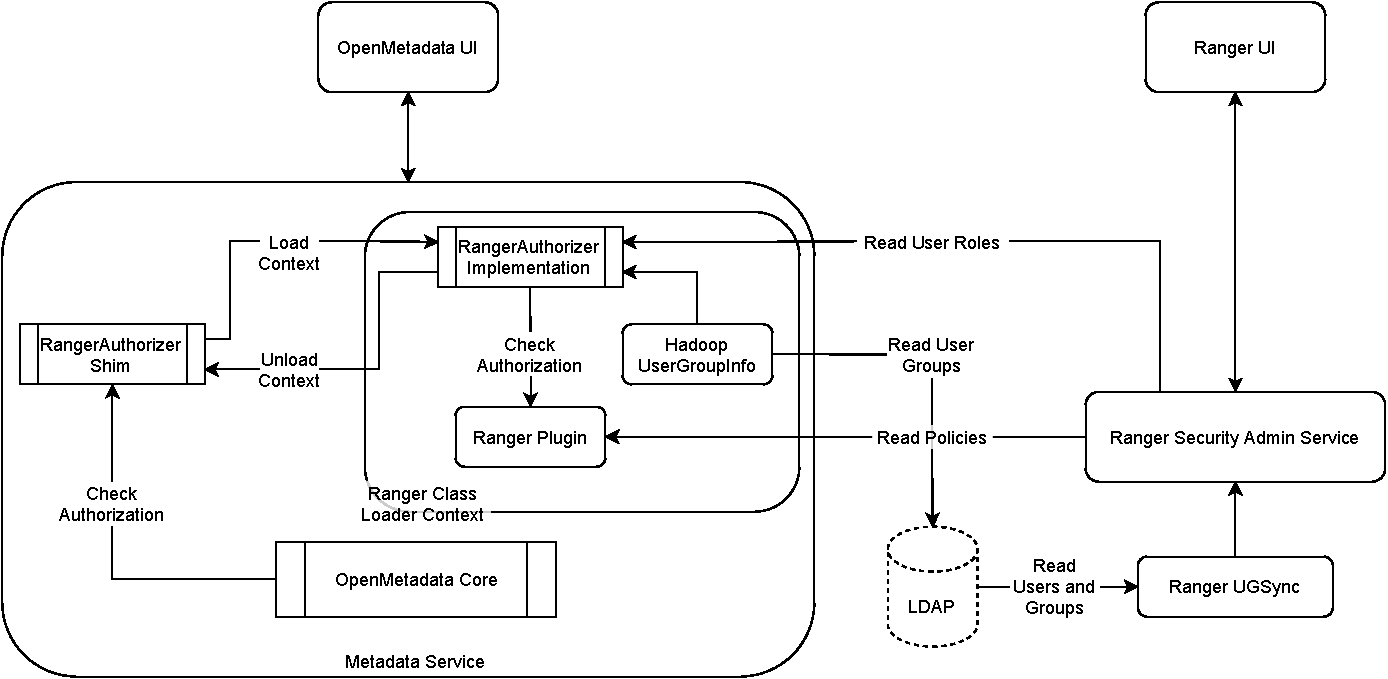
\includegraphics[width=0.8\textwidth]{chapters/design/figures/openmetadata-ranger-arch.pdf}
    \caption{High-level architectural overview of OpenMetadata and Apache Ranger system integration.}
    \label{fig:openmetadata-ranger-arch}
\end{figure}

\begin{figure}
    \centering
    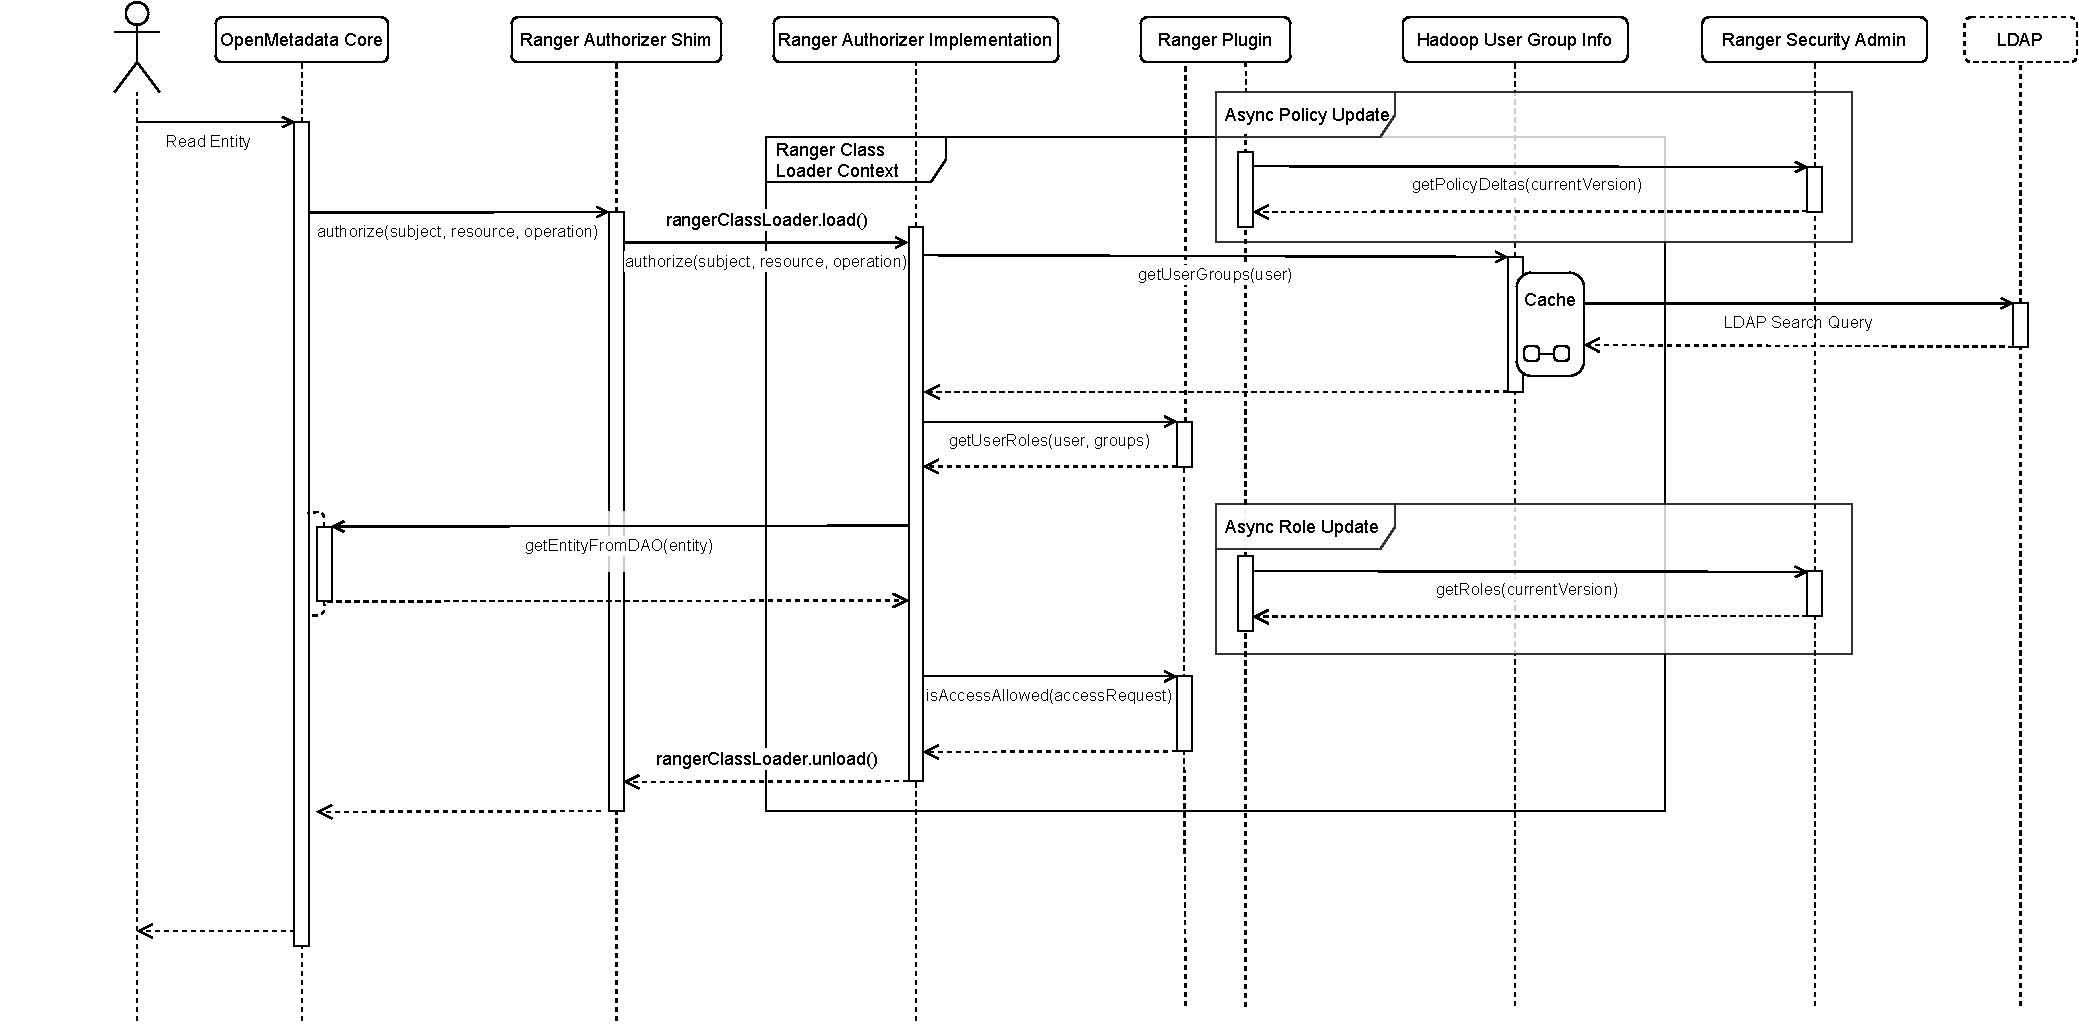
\includegraphics[width=\textwidth]{chapters/design/figures/openmetadata-ranger-lifecycle.pdf}
    \caption{High-level lifecycle of an  OpenMetadata authorisation request using Apache Ranger.}
    \label{fig:openmetadata-ranger-lifecycle}
\end{figure}

We begin by defining all the primary components of the system:

\begin{itemize}
    \item \textbf{OpenMetadata Core} - core OpenMetadata systems that handle loading entities from the Metadata Store, processing requests and calling the access control system when needed;
    \item \textbf{Ranger Authorizer Shim} - lightweight shim class that mediates calls to OpenMetadata's Ranger Authorizer Implementation by loading and unloading the class loader context;
    \item \textbf{Ranger Authorizer Implementation} - working components that use Apache Ranger libraries to handle authorization;
    \item \textbf{Hadoop User Group Information} - a configured instance of Hadoop libraries for reading a user's groups from an Active Directory or LDAP system;
    \item \textbf{Ranger Plugin} - a configured instance of the Apache Ranger policy evaluation libraries;
    \item \textbf{Ranger Security Admin Service}, \textbf{Ranger UGSync}, \textbf{LDAP} - same as previous definitions.
\end{itemize}

Figure \ref{fig:openmetadata-ranger-arch} illustrates the logical layout of components and how these communicate with each other. OpenMetadata Core is the entry point into the system and initialises authorisation requests. Ranger UGSync is complement asynchronous, running on an internal timer independent of events in the system. The OpenMetadata Core, Ranger Auhorizer Shim, Ranger Authozier Implementation, Hadoop User Group Information libraries and Ranger Plugin libraries are part of the same Java process, namely the Metadata Service. Still, the latter three are isolated in a Java class loader context that is unavailable to other components and is only accessible through the shim class.

Figure \ref{fig:openmetadata-ranger-lifecycle} represents the authorisation lifecycle of a read request sent by a user (directly through the API or through the UI) to OpenMetadata and how the various components communicate. The time axis (the vertical axis) is not to scale. 

OpenMetadata Core initiates an authorisation request by calling the Shim class, which loads the Ranger Class Loader Context and passes the call to the Ranger Authorizer Implementation. Evaluating the authorisation request has four steps: querying user groups from the Hadoop User Group Info provider, getting the roles based on the user and groups from the Ranger Plugin, loading the entity data from OpenMetadata Core (if not already provided) and finally, using the Ranger Plugin to check access. Once access has been decided, it returns and gives control to the Shim, which unloads the Ranger Class Loader Context and returns to the Core.

Hadoop User Group Info hits LDAP, the centralised user and groups database, and uses an in-memory cache to store results. Ranger Plugin keeps in-memory records of the policies and roles, asynchronously querying the Ranger Security Admin Service to update these.

This architecture combines synchronous and asynchronous operations and expensively uses in-memory duplication of remote resources to improve performance and avoid, as much as possible, calling external services in the critical path of access control evaluation.

\section{Service definition for OpenMetadata service types in Apache Ranger}

As discussed in Section \ref{sec:plugins_for_apache_ranger}, Apache Ranger requires a definition of the structure of OpenMetadata services, its resource types, access types, configuration properties and the implementation class. 

% We now focus on the resource types tree and access types.

OpenMetadata already defines internal resource names and access types the included access control system uses in the \mintinline[breaklines, breakbefore=/]{java}{openmetadata-serivce/src/main/resources/json.data/ResourceDescriptors.json} file found in the source code. The Apache Ranger service definition will follow the same naming scheme and implement a similar structure to maintain consistency. OpenMetadata resource names use camel casing (e.g., \mintinline{text}{databaseService}), which is not supported by Apache Ranger resource names as these do not accept capital letters, so a conversion to underscore case is applied (e.g., \mintinline{text}{database_service}).

The complete service definition for OpenMetadata services in Apache Ranger is provided in Appendix \ref{cha:servicedef_full}. It is also available in the \mintinline[breaklines, breakbefore=/]{java}{agent-common/src/main/resources/service-defs/ranger-servicedef-openmetadata.json} file in the Apache Ranger source code.

\subsection{Resource Types}

The resource tree is built using the resource types defined by OpenMetadata. A virtual root node that holds no that is used. One-to-many relationships between parent and child resource types give the hierarchy. Listing \ref{listing:tree_openmetadata_resources} provides a graphical representation of the resource tree.

OpenMetadata does not currently use the Feed resource type, but it is included here for forwards-compatibility. Tag and Glossary Term resources are recursive.

\begin{listing}
    
    \renewcommand\DTstyle{\rmfamily}
    \dirtree{%
    .1 Root. 
    .2 Database Service \DTcomment{\mintinline{text}{databaseService}}.
    .3 Database \DTcomment{\mintinline{text}{database}}.
    .4 Database Schema \DTcomment{\mintinline{text}{databaseSchema}}.
    .5 Table \DTcomment{\mintinline{text}{table}}.
    .2 Dashboard Service \DTcomment{\mintinline{text}{dashboardService}}.
    .3 Dashboard \DTcomment{\mintinline{text}{dashboard}}.
    .3 Chart \DTcomment{\mintinline{text}{chart}}.
    .2 Messaging Service \DTcomment{\mintinline{text}{messagingService}}.
    .3 Topic \DTcomment{\mintinline{text}{topic}}.
    .2 Machine Learning Service \DTcomment{\mintinline{text}{mlService}}.
    .3 Machine Learning Model \DTcomment{\mintinline{text}{mlModel}}.
    .2 Pipeline Service \DTcomment{\mintinline{text}{pipelineService}}.
    .3 Pipeline \DTcomment{\mintinline{text}{pipeline}}.
    .2 Storage Service \DTcomment{\mintinline{text}{storageService}}.
    .3 File Location \DTcomment{\mintinline{text}{location}}.
    .2 Metadata Service \DTcomment{\mintinline{text}{metadataService}}.
    .2 Glossary \DTcomment{\mintinline{text}{glossary}}.
    .3 Glossary Term \DTcomment{\mintinline{text}{glossaryTerm}}.
    .4 Glossary Term.
    .5 $\vdots$.
    .2 Tag Category \DTcomment{\mintinline{text}{tagCategory}}.
    .3 Tag \DTcomment{\mintinline{text}{tag}}.
    .4 Tag.
    .5 $\vdots$.
    .2 Bot \DTcomment{\mintinline{text}{bot}}.
    .2 Ingestion Pipeline \DTcomment{\mintinline{text}{ingestionPipeline}}.
    .2 User \DTcomment{\mintinline{text}{user}}.
    .2 Tams \DTcomment{\mintinline{text}{team}}.
    .2 Events \DTcomment{\mintinline{text}{events}}.
    .2 Feed \DTcomment{\mintinline{text}{feed}}.
    .2 Webhook \DTcomment{\mintinline{text}{webhook}}.
    .2 Custom Type \DTcomment{\mintinline{text}{type}}.
    .2 Test Suite \DTcomment{\mintinline{text}{testSuite}}.
    .3 Test Case \DTcomment{\mintinline{text}{testCase}}.
    .2 Web Analytic Event \DTcomment{\mintinline{text}{webAnalyticEvent}}.
    .2 Web Insight Chart \DTcomment{\mintinline{text}{webInsightChart}}.
    .3 KPI \DTcomment{\mintinline{text}{kpi}}.
    .2 Alert \DTcomment{\mintinline{text}{alert}}.
    .2 Alert Action \DTcomment{\mintinline{text}{alertAction}}.
    }

    \caption{Tree representation of OpenMetadata resource types.}
    \label{listing:tree_openmetadata_resources}
    
\end{listing}

\subsection{Access Types}

Access types define the operations that can be applied to resources. OpenMetadata utilises specialised access types to provide more precise access control for specific functions; e.g., the EditUsers access type enables adding or removing team members. 

Listing \ref{listing:tree_openmetadata_access_types} provides a graphical representation of the access types in OpenMetadata. The ViewAll and EditAll access types are shorthand for all view and edit operations. Unlike the tree of resource types, in the case of access types, a parent-child relationship does not imply ownership; thus, access types can be used independently of their parents.

Access types are not universally applicable to all resources type; each resource type specifies which access types can be used on it, e.g., Team resources support Create, Delete, ViewAll, EditAll, EditDisplayName, EditCustomFields and EditUsers operations. In contrast, Tables resources support all operations except EditUsers and EditStatus.

\begin{listing}

    \renewcommand\DTstyle{\rmfamily}
    \dirtree{%
    .1 All.
    .2 Create.
    .2 Delete.
    .2 ViewAll.
    .2 ViewBasic.
    .3 ViewUsage.
    .3 ViewTests.
    .3 ViewQueries.
    .3 ViewDataProfile.
    .3 ViewSampleData.
    .2 EditAll.
    .3 EditDescription.
    .3 EditDisplayName.
    .3 EditTags.
    .3 EditOwner.
    .3 EditTier.
    .3 EditCustomFields.
    .3 EditLineage.
    .3 EditStatus.
    .3 EditReviewers.
    .3 EditTests.
    .3 EditQueries.
    .3 EditDataProfile.
    .3 EditSampleData.
    .3 EditUsers.
    }

    \caption{Tree representation of OpenMetadata access types.}
    \label{listing:tree_openmetadata_access_types}
    
\end{listing}